\documentclass[11pt]{article}

\usepackage[margin=1in]{geometry}
\usepackage{amsmath,amssymb,mathtools}
\usepackage{booktabs}
\usepackage{hyperref}
\usepackage{xcolor}
\usepackage{tikz}
\usetikzlibrary{arrows.meta,positioning}

\title{Published Work on Trend Filtering on Graphs\\and Its Relevance to \texttt{gflow}}
\author{gflow graph trend filtering notes}
\date{\today}

\newcommand{\R}{\mathbb{R}}
\newcommand{\argmin}{\operatorname*{arg\,min}}

\begin{document}
\maketitle

\section{Short Answer}

Yes: graph trend filtering exists, is published, and is directly relevant to
the proposed \texttt{gflow} graph trend filtering project. The central paper is
\emph{Trend Filtering on Graphs} by Yu-Xiang Wang, James Sharpnack, Alex Smola,
and Ryan Tibshirani. It appeared first around AISTATS 2015 and then in JMLR
2016.

That paper generalizes one-dimensional trend filtering to arbitrary graphs by
penalizing the \(\ell_1\) norm of discrete graph differences. This is exactly
the graph analogue of the mechanism that made one-dimensional trend filtering
perform strongly in our path-graph benchmark: the method is locally adaptive,
because an \(\ell_1\) penalty can set many graph differences exactly to zero
while allowing selected nonsmooth changes.

\section{The Core Estimator}

Let \(G=(V,E)\) be an undirected graph with \(n=|V|\) vertices. A graph signal
is a vector
\[
\beta = (\beta_1,\ldots,\beta_n)^T \in \R^n,
\]
where \(\beta_i\) is the fitted value at vertex \(i\). Given noisy observations
\[
y = (y_1,\ldots,y_n)^T,
\]
graph trend filtering estimates \(\beta\) by solving
\[
\widehat\beta
=
\argmin_{\beta\in\R^n}
\left\{
\frac{1}{2}\|y-\beta\|_2^2
+
\lambda \|\Delta^{(k+1)}\beta\|_1
\right\}.
\]

The two terms have different jobs:
\begin{itemize}
  \item \(\frac{1}{2}\|y-\beta\|_2^2\) keeps the fitted graph signal close to
  the observed response.
  \item \(\lambda\|\Delta^{(k+1)}\beta\|_1\) penalizes graph roughness.
\end{itemize}

The key feature is the \(\ell_1\) norm. As in ordinary lasso, an \(\ell_1\)
penalty encourages sparsity. But here the sparse quantities are not regression
coefficients. They are graph differences of the fitted signal.

\section{The \(k=0\) Case: Graph Fused Lasso}

Choose an arbitrary orientation for every undirected edge. If an edge
\(e=(i,j)\) is oriented from \(i\) to \(j\), the oriented incidence matrix
\(D\) has one row per edge and one column per vertex:
\[
D_{e,i}=-1,\qquad D_{e,j}=1,\qquad D_{e,\ell}=0\quad(\ell\notin\{i,j\}).
\]
Then
\[
(D\beta)_e = \beta_j-\beta_i.
\]

For \(k=0\), graph trend filtering uses
\[
\Delta^{(1)} = D.
\]
Therefore the penalty is
\[
\|\Delta^{(1)}\beta\|_1
=
\|D\beta\|_1
=
\sum_{e=(i,j)\in E} |\beta_i-\beta_j|.
\]

The optimization problem becomes
\[
\widehat\beta
=
\argmin_{\beta\in\R^n}
\left\{
\frac{1}{2}\|y-\beta\|_2^2
+
\lambda \sum_{(i,j)\in E}|\beta_i-\beta_j|
\right\}.
\]
This is graph fused lasso, also called graph total variation denoising.

Intuitively, the method encourages neighboring vertices to have equal fitted
values, but it allows jumps on selected edges when the data strongly support
them. Thus the fitted graph signal is often piecewise constant over graph
regions.

\section{Higher-Order Graph Trend Filtering}

Let
\[
L = D^T D
\]
be the graph Laplacian. Wang, Sharpnack, Smola, and Tibshirani define
higher-order graph difference operators by alternating incidence-like and
Laplacian-like operations:
\[
\Delta^{(k+1)}
=
\begin{cases}
L^{(k+1)/2}, & k \text{ odd},\\[1mm]
D L^{k/2}, & k \text{ even}.
\end{cases}
\]

This gives a sequence of graph analogues of one-dimensional trend filtering:

\begin{center}
\begin{tabular}{lll}
\toprule
Order \(k\) & Penalty & Interpretation\\
\midrule
\(0\) & \(\|D\beta\|_1\) & edge jumps; piecewise constant signal\\
\(1\) & \(\|L\beta\|_1\) & graph Laplacian values; piecewise linear analogue\\
\(2\) & \(\|D L\beta\|_1\) & edge differences of graph Laplacian values; piecewise quadratic analogue\\
\bottomrule
\end{tabular}
\end{center}

The words ``piecewise linear'' and ``piecewise quadratic'' are exact on a path
graph and analogical on a general graph. On a general graph, there is no single
left-to-right coordinate system. The operator nevertheless plays the same role:
it measures higher-order graph roughness and uses an \(\ell_1\) penalty to make
that roughness sparse.

\section{Visual Intuition}

\begin{figure}[ht]
\centering
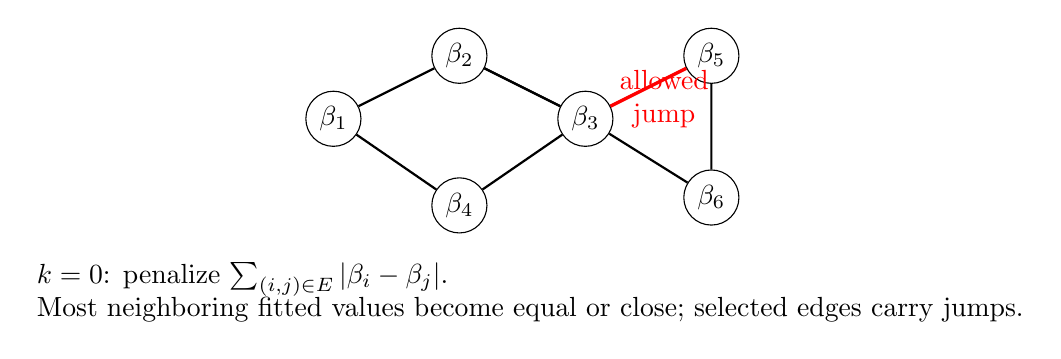
\begin{tikzpicture}[scale=1.0,>=Latex]
  \tikzstyle{vtx}=[circle,draw,minimum size=7mm,inner sep=0pt]
  \node[vtx] (a) at (0,1.2) {\(\beta_1\)};
  \node[vtx] (b) at (1.6,2.0) {\(\beta_2\)};
  \node[vtx] (c) at (3.2,1.2) {\(\beta_3\)};
  \node[vtx] (d) at (1.6,0.1) {\(\beta_4\)};
  \node[vtx] (e) at (4.8,2.0) {\(\beta_5\)};
  \node[vtx] (f) at (4.8,0.2) {\(\beta_6\)};

  \draw[thick] (a)--(b)--(c)--(d)--(a);
  \draw[thick] (c)--(e)--(f)--(c);
  \draw[thick] (b)--(c);

  \draw[red,very thick] (c)--(e);
  \node[red,align=center] at (4.2,1.45) {allowed\\jump};

  \node[align=left] at (2.5,-1.0) {
    \(k=0\): penalize \(\sum_{(i,j)\in E}|\beta_i-\beta_j|\).\\
    Most neighboring fitted values become equal or close; selected edges carry jumps.
  };
\end{tikzpicture}
\caption{Graph fused lasso, the \(k=0\) graph trend filtering case, encourages
piecewise constant graph regions separated by a small number of active edges.}
\end{figure}

\section{Why This Matters for \texttt{gflow}}

The current metric graph low-pass smoother is an \(\ell_2\)-spectral smoother.
In its simplest unnormalized form, it is closely related to minimizing
\[
\sum_i (y_i-f_i)^2 + \eta f^T L f.
\]
This penalty smooths globally through the graph Laplacian. It suppresses
high-frequency components, but the penalty is quadratic and therefore tends to
spread smoothing everywhere.

Graph trend filtering would be the \(\ell_1\)-adaptive counterpart:
\[
\sum_i (y_i-\beta_i)^2
+
\lambda \|\Delta^{(k+1)}\beta\|_1.
\]
Because the penalty is \(\ell_1\), the fitted signal can be smooth or simple
over most of the graph while preserving localized changes where the data
support them.

This makes graph trend filtering a natural comparator to:
\begin{itemize}
  \item \texttt{fit.metric.graph.lowpass()}, the metric-conductance graph
  low-pass smoother;
  \item \texttt{fit.rdgraph.regression()}, the existing
  Riemannian-complex/overlap-density graph smoother;
  \item one-dimensional \texttt{genlasso::trendfilter()}, when the graph is a
  path graph.
\end{itemize}

\section{Weighted Graphs and Metric Conductances}

The canonical graph trend filtering paper is often presented using an
unweighted incidence matrix \(D\). For a weighted graph, a natural extension is
to use a weighted incidence operator. If \(e=(i,j)\), one can define
\[
(D_w\beta)_e = \omega_e(\beta_j-\beta_i).
\]
Then the \(k=0\) penalty becomes
\[
\|D_w\beta\|_1
=
\sum_{e=(i,j)\in E}\omega_e|\beta_i-\beta_j|.
\]

If the graph has conductances \(c_e\), there are at least two plausible
conventions:
\[
(D_w\beta)_e = c_e(\beta_j-\beta_i)
\]
or
\[
(D_w\beta)_e = \sqrt{c_e}(\beta_j-\beta_i).
\]

The square-root convention aligns with the quadratic Laplacian identity
\[
\|D_w\beta\|_2^2 = \beta^T L_w \beta
\quad\text{when}\quad
L_w = D_w^T D_w.
\]
The linear-conductance convention makes the \(\ell_1\) edge penalty scale
directly as
\[
\sum_e c_e|\beta_i-\beta_j|.
\]

For \texttt{gflow}, this is a genuine modeling decision. Since
\texttt{fit.metric.graph.lowpass()} already transforms metric edge lengths
\(\ell_e\) into conductances \(c_e=\phi(\ell_e)\), a graph trend filtering
comparator should probably expose the weighting rule explicitly rather than
burying it inside the solver.

\section{Related Published Work}

\subsection*{Trend Filtering on Graphs}

Yu-Xiang Wang, James Sharpnack, Alex Smola, and Ryan J. Tibshirani.
\emph{Trend Filtering on Graphs}. JMLR, 2016.

\begin{itemize}
  \item arXiv: \url{https://arxiv.org/abs/1410.7690}
  \item JMLR PDF: \url{https://jmlr.csail.mit.edu/papers/volume17/15-147/15-147.pdf}
  \item Main contribution: graph trend filtering estimator and theory.
\end{itemize}

\subsection*{The DFS Fused Lasso}

Oscar Hernan Madrid Padilla, James Sharpnack, James G. Scott, and Ryan J.
Tibshirani. \emph{The DFS Fused Lasso: Linear-Time Denoising over General
Graphs}. JMLR, 2018.

\begin{itemize}
  \item JMLR page: \url{https://www.jmlr.org/beta/papers/v18/16-532.html}
  \item Main contribution: scalable graph fused lasso / graph total variation
  denoising, mostly corresponding to the \(k=0\) case.
\end{itemize}

\subsection*{Fused \(\ell_1\) Trend Filtering on Graphs}

Vladimir Pastukhov. \emph{Fused \(\ell_1\) Trend Filtering on Graphs}. arXiv,
2024.

\begin{itemize}
  \item arXiv: \url{https://arxiv.org/abs/2401.05250}
  \item Main contribution: fused graph trend filtering with additional
  fusion-style regularization and computationally feasible iterative solvers.
\end{itemize}

\section{Suggested \texttt{gflow} Starting Point}

The first implementation should probably start with weighted graph fused lasso:
\[
\widehat\beta
=
\argmin_{\beta\in\R^n}
\left\{
\frac{1}{2}\|y-\beta\|_2^2
+
\lambda \|D_w\beta\|_1
\right\}.
\]
This is the \(k=0\) graph trend filtering case. It is easier to test and
interpret than higher-order graph trend filtering, and it forces us to settle
the key package questions:
\begin{itemize}
  \item graph canonicalization;
  \item edge orientation;
  \item metric length to conductance transforms;
  \item weighted incidence convention;
  \item lambda grid and tuning behavior;
  \item return object structure.
\end{itemize}

Once that is stable, higher-order graph trend filtering can be introduced:
\[
\widehat\beta
=
\argmin_{\beta\in\R^n}
\left\{
\frac{1}{2}\|y-\beta\|_2^2
+
\lambda \|\Delta_w^{(k+1)}\beta\|_1
\right\}.
\]

\end{document}
